\documentclass[a4paper,12pt,titlepage]{article}
\usepackage[left=2cm,top=3cm,right=2cm,bottom=1cm,head=2.0cm,includefoot]{geometry}
\usepackage[spanish,activeacute]{babel}
\usepackage{graphicx}
\usepackage{fancyhdr}
\usepackage{pdfpages}
\title{\textbf{Tejedur\'{i}a Dolly S.A.}}
\author{\textbf{Grupo B1}}
\begin{document} 
\pagestyle{fancy}
\chead{Grupo B1}
\lhead{
\includegraphics[width=1.7cm]{./logo1.png}}
\lfoot{71.12 - Estructura de las Organizaciones}
\rfoot{$1^{er}$ Cuatrimestre 2011}
\maketitle
\tableofcontents


\newpage
\section{\underline{Enunciado}}
Este ejemplo ha sido tomado de un caso real, al cual se le han practicado algunas
simplificaciones para convertirlo en un caso al que se le pueden aplicar las t\'{e}cnicas
de organizaci\'{o}n.\\
Tejedur\'{i}a DOLLY es una empresa dedicada a la fabricaci\'{o}n de prendas de tejido
de punto partiendo de hilados de fibras naturales, artificiales y/o sus mezclas.
Es una empresa Pyme caracter\'{i}stica de nuestro pa\'{i}s, en la cual se ha puesto mas
voluntarismo que aplicaci\'{o}n de m\'{e}todos cient\'{i}ficos o profesionalizados
La empresa es del tipo familiar, con conformaci\'{o}n legal de Sociedad An\'{o}nima, en
la cual el \'{u}nico director, que trabaja como gerente operativo, es un profesional de
Ingenier\'{i}a, y ha dirigido esta empresa en los \'{u}ltimos 6 a\~nos.
La empresa comercializa sus productos en el mercado local, el 90\% a trav\'{e}s de 10
negocios propios, y un 10\% a trav\'{e}s de distribuidores o negocios que compran
directamente en el deposito.\\
Los diez locales est\'{a}n distribuidos en Capital, Gran Buenos Aires, La Plata,
C\'{o}rdoba, Mar del Plata y Mendoza. Los negocios tienen de dos a cuatro
empleadas, de las cuales, una de ellas, es la encargada del negocio. En total el
plantel de vendedoras es de 45 personas.\\
Hay un jefe de ventas que supervisa, la venta de los locales, la venta mayorista y
tambi\'{e}n tiene a su cargo el dep\'{o}sito de productos terminados.\\
La empresa cuenta con un sistema inform\'{a}tico que interconecta los locales con la
f\'{a}brica, que por ser un sistema un tanto r\'{i}gido sufre a menudo problemas que
impiden que la informaci\'{i}on sobre ventas, stock y pedidos de los clientes se
actualicen correctamente.\\
Esto genera inconvenientes en las tiendas, que pueden quedar desabastecidas o
sobrestockeadas, adem\'{a}s de generar inconvenientes contables.\\ \\
Las ventajas competitivas de la empresa son trabajar con materia prima de calidad,
en este caso importada de una importante firma Italiana, manteniendo un contrato
de exclusividad para la regi\'{o}n, esto otorga una diferenciaci\'{o}n en los productos
finales.\\
La segunda ventaja es ser una f\'{a}brica de tejido de punto integrada verticalmenete
hasta llegar al consumidos, caracteristica que es poco comun
Dolly Fabrica prendas con alto contenido de dise\~no con lo que ha logrado
imponerse en un mercado dif\'{i}cil. Nuestro an\'{a}lisis se realiza a mediados del a\~no
2000 donde lo \'{u}nico que pod\'{i}amos asegurar es que el tan pronosticado Y2K
fueron solo amenazas.\\
Al ser prendas de dise\~no se realizan en cantidades chicas 500 a 2000 unidades
con excepci\'{o}n de algunos comoditis, que se hacen de a 5000 unidades y se
repiten producciones.\\
Deben agregar a esto que cada partida se ti\~nen de 4 o 5 colores diferentes
Todos los a\'~nos , el dise\~nador y el due\~no de la empresa viajan a Europa para
relevar las tendencias esteticas, en modelos y colores dado que estando en
contraestaci\'{o}n, esto le permite definir anticipadamente la producci\'{o}n de cada
temporada. Esto, agregado a la relaci\'{o}n precio-calidad, resultante de su m\'{e}todo
de comercializaci\'{o}n pone a la empresa entre las mas importantes del mercado
La empresa tiene un negocio donde vende mercader\'{i}a de dise\~nos esclusivos y
muy cuidada calidad orientado a boutiques de alta costura, para lo cual cada
temporada, organiza un desfile con su correspondiente organizaci\'{o}n. El resto de
los negocios venden productos con un dise\~no Standard de acuerdo a las
necesidades del mercado al cual va dirigido.\\
En este caso tambi\'{e}n tienen muy buena acogida, logrando vender importantes
cantidades y con un nivel de ventas que si bien tiene picos se mantienen todo el
a\~no manteniendo la operaci\'{o}n de los locales a pleno.\\ \\
La empresa, en vista del \'{e}xito comercial que ten\'{i}a, y esperando mejorar la calidad
y la productividad, en el a\~no 1998 compr\'{o} maquinas de una nueva tecnolog\'{i}a para
reemplazar las antiguas maquinas. Estas maquinas producen prendas con la forma
exacta que debe tener cada pieza, evitando la operaci\'{o}n de corte y todo el
desperdicio de material que se produce al cortar con los moldes los pa\~nos de tejido
Desgraciadamente no se tomaron las precauciones de tomar personal capacitado
para el manejo de esas maquinas (o capacitar personal propio) y estas no solo no
lograban la productividad Standard sino que exist\'{i}an muchos desperdicios de
puesta a punto o de programas mal desarrollados. Tambi\'{e}n se produc\'{i}an
problemas de barrado (que es una l\'{i}nea en el tejido debido a diferencia de tensi\'{o}n)
Si bien se aumento la producci\'{o}n total con estas maquinas, no fue en la cantidad
que se esperaba y el 70\% .del tejido era realizada por las viejas maquinas
circulares.\\
Estas m\'{a}quinas adem\'{a}s como fueron compradas con credito a 5 a\~nos produc\'{i}an
una erogaci\'{o}n mensual mayor que la ganancia que se produc\'{i}a por su uso
La fabrica se encuentra en el gran Buenos Aires, y desarrolla sus actividades en un
edificio alquilado de 4000 m2. Compra hilado de pelo (un tipo de lana) y algod\'{o}n
seg\'{u}n la temporada, el 60\% de esta materia prima es importada de Italia. El hilado
es la principal de las materias primas, al que le corresponde un porcentaje
importante del total de las compras.\\ 
A continuaci\'{o}n se hace un a breve descripci\'{o}n de la empresa y su proceso
productivo.\\ \\

\textbf{2- RELEVAMIENTO DEL PROCESO PRODUCTIVO}\\ \\
El proceso productivo est\'{a} dividido en siete sectores consecutivos a trav\'{e}s de los
cuales se va transformando la materia prima hasta obtener el producto terminado,
embalado y puesto a disposici\'{o}n del dep\'{o}sito de productos terminados. La
distribuci\'{o}n en planta es por procesos y los sectores son:\\

\begin{enumerate}
 \item Dep\'{o}sito de materias primas.
 \item Tejedur\'{i}a: 
\begin{itemize}
 \item Enconado
 \item Tejido
 \item Lavado
\end{itemize}
 \item Corte
 \item Confecci\'{o}n
 \item Tintorer\'{i}a
 \item Terminaci\'{o}n
 \item Expedici\'{o}n
\end{enumerate}

En algunos casos, estos procesos son llevados a cabo a trav\'{e}s de terceros, seg\'{u}n
su naturaleza y los planes de producci\'{o}n. Las empresas proveedoras de estos
servicios son llamadas ``fasones'' o \``terceros''
El proceso de ``Tintorer\'{i}a'' que en realidad es el te\~nido de las prendas se realiza
cuando corresponde, y es siempre tercerizado puesto que TEJEDURIA DOLLY no
posee instalaciones para tal fin.\\

\begin{center}\textbf{\underline{Descripci\'{o}n de cada proceso.}}\end{center}
\textbf{\underline{2.1- Dep\'{o}sito de MP.}} 
 -\\ \\
\textbf{\underline{2.2- Tejedur\'{i}a:}}\\
El sector de tejedur\'{i}a se compone de tres partes\\
\underline{2.2.A- Enconado:} Los conos de hilado se re-enconan en casi todos los casos con
el fin de lograr una tensi\'{o}n pareja y acorde a los requerimientos de cada telar. En
el mismo proceso se eliminan nudos y aglomeraciones de fibras y se le aplica
parafina s\'{a}lida al hilado, para facilitar su tejido.\\
\underline{2.2.B- Tejedur\'{i}a:} Este es el proceso fundamental y caracter\'{i}stico de la empresa.
Se teje en los telares seg\'{u}n especifican las \'{o}rdenes de producci\'{o}n y las fichas de
producto.\\
Las partidas que no contin\'{u}en su proceso en el sector de lavado, se someten aqu\'{i}
a un control estad\'{i}stico de calidad.\\
\underline{2.2.C- Lavadero:} Mediante este proceso se lavan las piezas tejidas en una soluci\'{o}n
acuosa de distintos agentes detergentes y humectantes. Luego se las centrifuga y
finalmente se las seca con aire caliente. La finalidad de este proceso es
fundamentalmente la de lograr una estabilidad dimensional y una eliminaci\'{o}n de
las tensiones internas adquiridas durante el tejido.\\
Las partidas listas para continuar el proceso son sometidas aqu\'{i} a un control
estad\'{i}stico de calidad\\
\textbf{\underline{2.3- Corte.}}\\
Para la obtenci\'{o}n de diversas formas a partir de piezas de forma rectangular, se
recortan los pa\~nos tejidos seg\'{u}n las formas y dimensiones especificadas en las
planillas de producto y el encogimiento previsto durante el proceso de te\~nido.
Luego de cortadas, las piezas se ordenan por tipo de pieza, se atan y se identifican
claramente los bultos. Las partidas ya cortadas se estiban en las estanter\'{i}as si van
a ser confeccionadas por el sector de confecci\'{o}n y se embolsan si es que van a ser
confeccionadas por talleres de terceros. Estas bolsas se apilan en forma separada.\\
\textbf{\underline{2.4- Confecci\'{o}n}}\\
Las distintas piezas tejidas que componen una prenda se unen aqu\'{i} mediante
distintos tipos de costura. Esto se hace siguiendo las reglas de arte en la materia, y
en funci\'{o}n de las especificaciones consignadas en las fichas de cada producto.
Para la confecci\'{o}n interna, la persona encargada del sector determina en funci\'{o}n
de la Ficha de Producto, que m\'{a}quina corresponde utilizar para cada una de las
costuras necesarias y que secuencia se seguir\'{a} hasta confeccionar todas las
prendas de la partida. La misma encargada se ocupa de la traslaci\'{o}n de los bultos
entre los diferentes puestos de trabajo, y de la entrega de las partidas ya
confeccionadas al sector de terminaci\'{o}n.\\
\textbf{\underline{2.5- Tintorería}}\\
Este trabajo se terceriza, pero exige un muy prolijo conteo de expedici\'{o}n y
recepci\'{o}n.\\
Este es el momento en que se toma la decisi\'{o}n respecto del color de las prendas.\\
Tareas previas al te\~nido:\\
\underline{ - Control de colores:} Se controla que los colores recibidos desde tintorer\'{i}a se
correspondan con la carta de colores prevista.\\
\textbf{\underline{2.6- Terminaci\'{o}n}}\\
Cuando las partidas est\'{a}n confeccionadas, la persona encargada del sector de
terminaci\'{o}n determina la secuencia de tareas a realizar sobre la prenda a los
efectos de dejarla lista para la venta. La siguiente es la secuencia general:\\
\textbf{\underline{2.7- Expedici\'{o}n}}\\
En este sector se almacenan las prendas para ser enviados en el momento
oportuno\\ \\
\textbf{3- DETALLES DEL PERSONAL}\\
El sector fabril se encuentra distribuido en las secciones anteriores que
detallaremos.\\
En RECEPCI\'{o}N DE MATERIAS PRIMAS Y OFICINA DE PRODUCCI\'{o}N se
trabaja un turno con dos personas.\\
En TEJEDUR\'{i}A existen dos encargados que supervisan el sector de ENCONADO
con dos operarios, TEJEDUR\'{i}A tiene 18 operarios y el LAVADERO que cuenta con
4 personas. Estos sectores trabajan dos turnos entre los que se divide el personal.
El sector de CORTE tiene un encargado con cuatro personas a cargo y
CONFECCI\'{o}N tiene un encargado, un ayudante y 18 operarias.\\
Por ultimo la encargada de TERMINACI\'{o}N tiene 14 operarias. De este sector la
mercader\'{i}a pasa a DEPOSITO que cuenta con un encargado y dos personas.
Aunque este ultimo sector depende del jefe de ventas.\\
La DIRECCI\'{o}N DE FABRICA est\'{a} a cargo de un jefe de producci\'{o}n y cuenta
como auxiliares con una persona de mantenimiento y un chofer.\\
Existe un sector de INGENIER\'{i}A Y CALIDAD con un encargado y dos personas a
su cargo.\\
Un JEFE DE OPERACIONES y producto con una encargada de medidas y puesta
a punto.\\
La ADMINISTRACI\'{o}N esta dirigida por un contador y se maneja con cuatro
personas, que tambi\'{e}n asisten al gerente.\\
El personal de f\'{a}brica eran unas 80 personas, mas el personal de los locales (50
empleados) y administrativos, de logistica y directivos agregaban 20 personas.
Ten\'{i}an una antiguedad promedio de 10 a\~nos y conoc\'{i}an bien su oficio, pero se
resist\'{i}an a los cambios tecnol\'{o}gicos.\\ \\
Incorporaci\'{o}n de sector.\\
En este momento (a\~no 2000) se dispuso incorporar un sector de calidad con el fin
de reducir el desperdicio que rondaba el 20\% (adicional a lo que se explico de los
telares computarizados. Pero esta tarea tampoco fue f\'{a}cil debido a que en la
industria textil se acostumbra a tener medidas aproximadas y el personal reclutado
no tenia la experiencia en el rubro como para liderar este cambio.\\ \\
\underline{Se pide} que planteen una estructura adecuada alternativa a la presentada y las
medidas que se deben poner en practica para mejorar la situaci\'{o}n problem\'{a}tica en
que se encuentra la empresa.
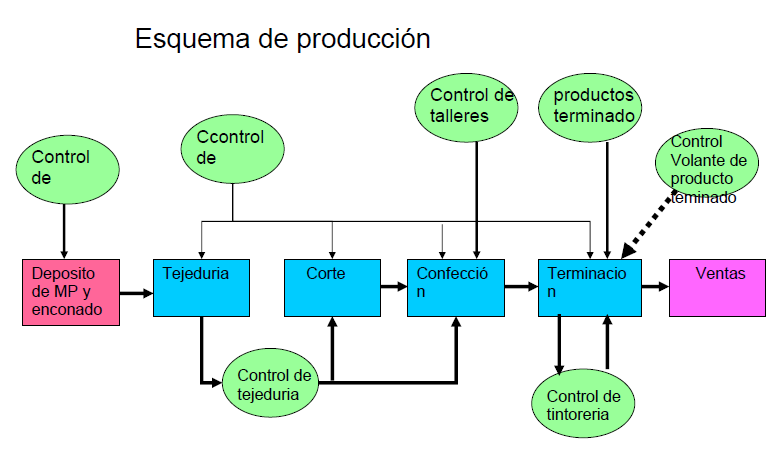
\includegraphics[width=400pt]{./esquemaproduccionDolly.png}



\newpage
\section{\underline{Desarrollo}}
	\subsection {Introducci\'{o}n a la empresa}
	Tejedur\'{i}a Dolly S. A. es una empresa Pyme de tipo familiar, con f\'{a}brica en Buenos Aires y locales en Capital, Gran Buenos Aires, La Plata, C\'{o}rdoba, Mar del Plata y Mendoza. Su director es un profesional de Ingenier\'{i}a.\\
	
	Dentro del rubro textil, se dedica a la fabricaci\'{o}n de prendas de tejido de punto a partir de hilados de fibras naturales, artificiales o bien sus mezclas.
Comercializa sus productos en el mercado local, en su mayor\'{i}a a trav\'{e}s de negocios propios (90\%) pero tambi\'{e}n mediante distribuidores y negocios que compran directamente en el dep\'{o}sito.

	\subsection {Ventajas}
	Al trabajar con materia prima de calidad, en este caso importada de una importante firma italiana (con un contrato de exclusividad para la regi\'{o}n), otorga una diferencia en los productos finales.\\
	
	Adem\'{a}s tiene la caracter\'{i}stica de ser una f\'{a}brica de tejido de punto integrada verticalmente hasta llegar al consumidor.\\
	
	El nivel de ventas, si bien tiene picos, mantiene todo el a\~no la operaci\'{o}n de los locales a pleno. Un factor que influye positivamente en esto es la adaptaci\'{o}n que se hace a las prendas para lograr su adecuaci\'{o}n a las tendencias est\'{e}ticas del momento, en cuanto a modelos y colores.
Por tanto, consecuencia de su m\'{e}todo de comercializaci\'{o}n es que la relaci\'{o}n precio-calidad ponga a la empresa entre las m\'{a}s importantes del mercado.

	\subsection {Aspectos Desfavorables}
	La rigidez del sistema inform\'{a}tico que interconecta los locales con la f\'{a}brica propensa retrasos y confusiones, debido a que impide la actualizaci\'{o}n inmediata de la informaci\'{o}n sobre ventas, stock y pedidos de los clientes. Esto resulta en detrimento de las tiendas: se producen circunstancias tanto de escasez como de abundancia de producto, adem\'{a}s de inconvenientes contables.\\
	
	Por otra parte, los desperfectos se ven potenciados por la falta de personal capacitado para manejar las nuevas m\'{a}quinas; si bien aument\'{o} la producci\'{o}n total, no s\'{o}lo no lleg\'{o} a alcanzarse la cantidad esperada sino que adem\'{a}s se ocasionaron desperdicios en la puesta a punto y deficiencias por programas mal desarrollados.


\newpage
\section{\underline{Organigrama actual de la empresa}}
	\begin{center}
	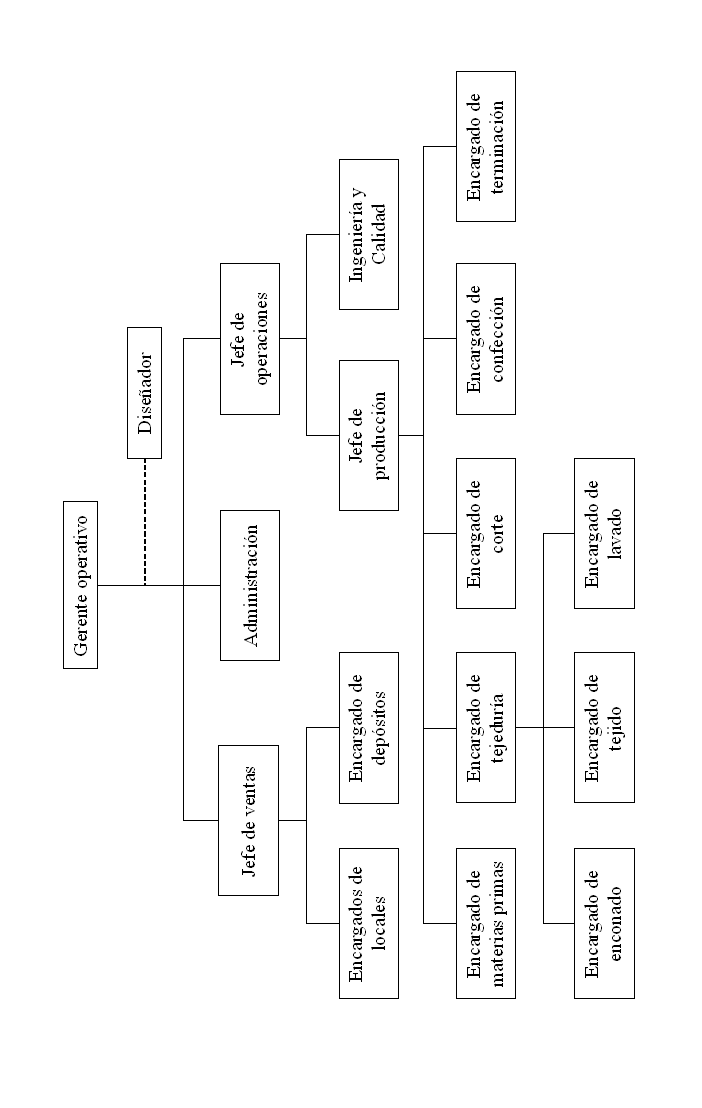
\includegraphics[width=450pt]{./DollyOrnigrama.png}
	\end{center}



\newpage
\section{\underline{An\'{a}lisis del caso}}
	\subsection{An\'{a}lisis}
	La empresa fue todo un \'exito y logr\'o posicionarse entre las mejores en su negocio. Cuenta con ventajas distintivas para hacerse resaltar, y ha logrado mantener un alto nivel de producci\'on que mantiene un nivel constante de ventas durante el a\~no. Otro punto a favor es que posee empleados con promedio de 10 a\~nos de antig\"uedad, por lo tanto son experimentados en sus \'areas de trabajo.\\
		
	Sin embargo, actualmente la empresa dos principales problemas:\\
	
	Por un lado est\'a la inserici\'on de maquinarias tecnol\'ogicamente avanzadas para aumentar la cantidad y calidad de producci\'on. \'Esto tuvo el efecto contrario, ya que los operarios no estaban capacitados para dichas m\'aquinas. Por otro lado esta el problema de conexi\'on entre la f\'abrica y los comercios de venta, que dificulta mantener un stock \'optimo.\\
	
	Una optimizaci\'on interesante ser\'ia incorporar instalaciones necesarias para realizar la etapa de tintorer\'ia en forma propia. Con esto se lograr\'ia que la producci\'on en ninguna parte dependa de un tercero.


	\subsection{Soluci\'on propuesta}
	En la empresa se observa una resistencia de los empleados a los cambios tecnol\'ogicos, esto es el causante de los dos grandes problemas antes mencionados. Hay que resolver esta cuesti\'on para que la empresa que de en \'optimas condiciones.\\

	Entonces, habr\'ia que capacitar a los empleados para que puedan utilizar y desenvolverse mejor no s\'olo con las maquinarias nuevas, sino tambi\'en con el sistema inform\'atico mejorado que se implementar\'a. \'Este \'ultimo es para mejorar la comunicaci\'on entre el dep\'osito y el personal de venta, para que se pueda transmitir correctamente y r\'apidamente los cambios en el stock. De esta forma, la empresa muestra tranquilidad a sus empleados y les hace ver que los cambios tecnol\'ogicos son un hecho positivo, y no una amenaza a sus puestos de trabajo. 


	\subsection{Matriz FODA}
	\vspace*{0.5cm}
	\begin{tabular}{|c|c|}
	\hline 
	\textbf{Fortalezas} & \textbf{Oportunidades} \\ \hline & \\
- Trabajar con materia prima de calidad. & - Avance tecnol\'{o}gico.\\ &\\
- Ser una f\'{a}brica de punto integrada & \\verticalmente hasta llegar al consumidor. &\\ &\\ & \\
- Estudio de las tendencias de moda. & \\& \\ & \\
- Excelente calidad de productos.& \\& \\

	\hline
	\textbf{Debilidades} & \textbf{Amenazas} \\
	\hline &\\
- Contar con un sistema inform\'{a}tico r\'{i}gido& - Entrada de nuevos competidores. \\que sufre continuos problemas que impide la &\\ actualizaci\'{o}n de la informaci\'{o}n. &\\ &\\
- Alto nivel de desperdicio en el procesamiento &\\ de la materia prima debido a los &\\ m\'{e}todos y maquinarias actuales. &\\ &\\
- Falta de capacitaci\'{o}n del personal para &\\el uso de las nuevas maquinarias. Esto &\\ produce p\'{e}rdida de rendimiento en las mismas. &\\ &\\
- Personal se resiste a cambios tecnol\'{o}gicos. &\\ &\\
	\hline    
	\end{tabular}


\newpage
\section{\underline{Organigrama de la soluci\'on propuesta}}
	\begin{center}
	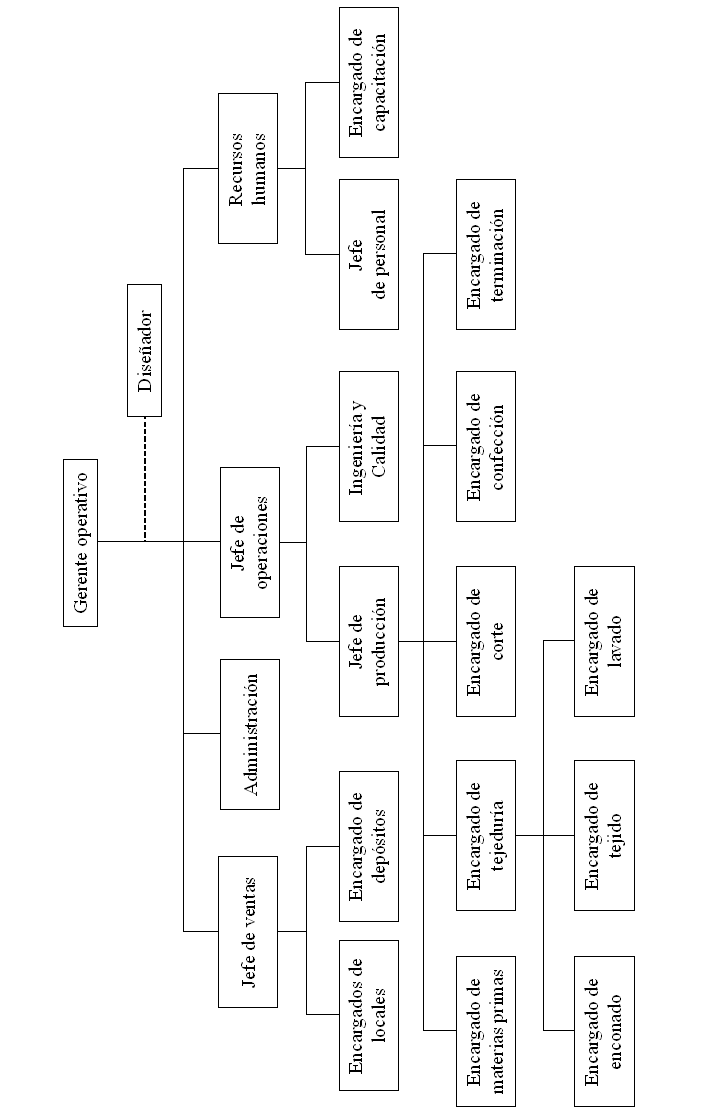
\includegraphics[width=430pt]{./DollyOrnigramaSolucion.png}
	\end{center}


\end{document}